\mysubsubsection{Optical Flow}

\noindent
%
We have chosen the Dimetrodon image pair from the Middlebury flow
dataset~\cite{middlebury_optical_flow}. Fig.~\ref{fig:optical_flow_convergence}
shows the energy plots of the three competing methods, Fusion Move
(FM), Parallel Fusion Move (PFM), and Hierarchical Fusion Move (HFM),
against our Swarm Fusion methods (SF-MF, SF-SS, SF). A key observation
is that SF-MF converges quicker and better than PFM. This is indeed the
benefits of solution sharing in our network. Optical flow is a more
difficult problem and many solution proposals are not effective.
The solution sharing (i.e., SF-MF) allows all the threads to exchange
effective solution proposals in the middle of the
optimization.

\begin{figure}[!h]
  \centering
  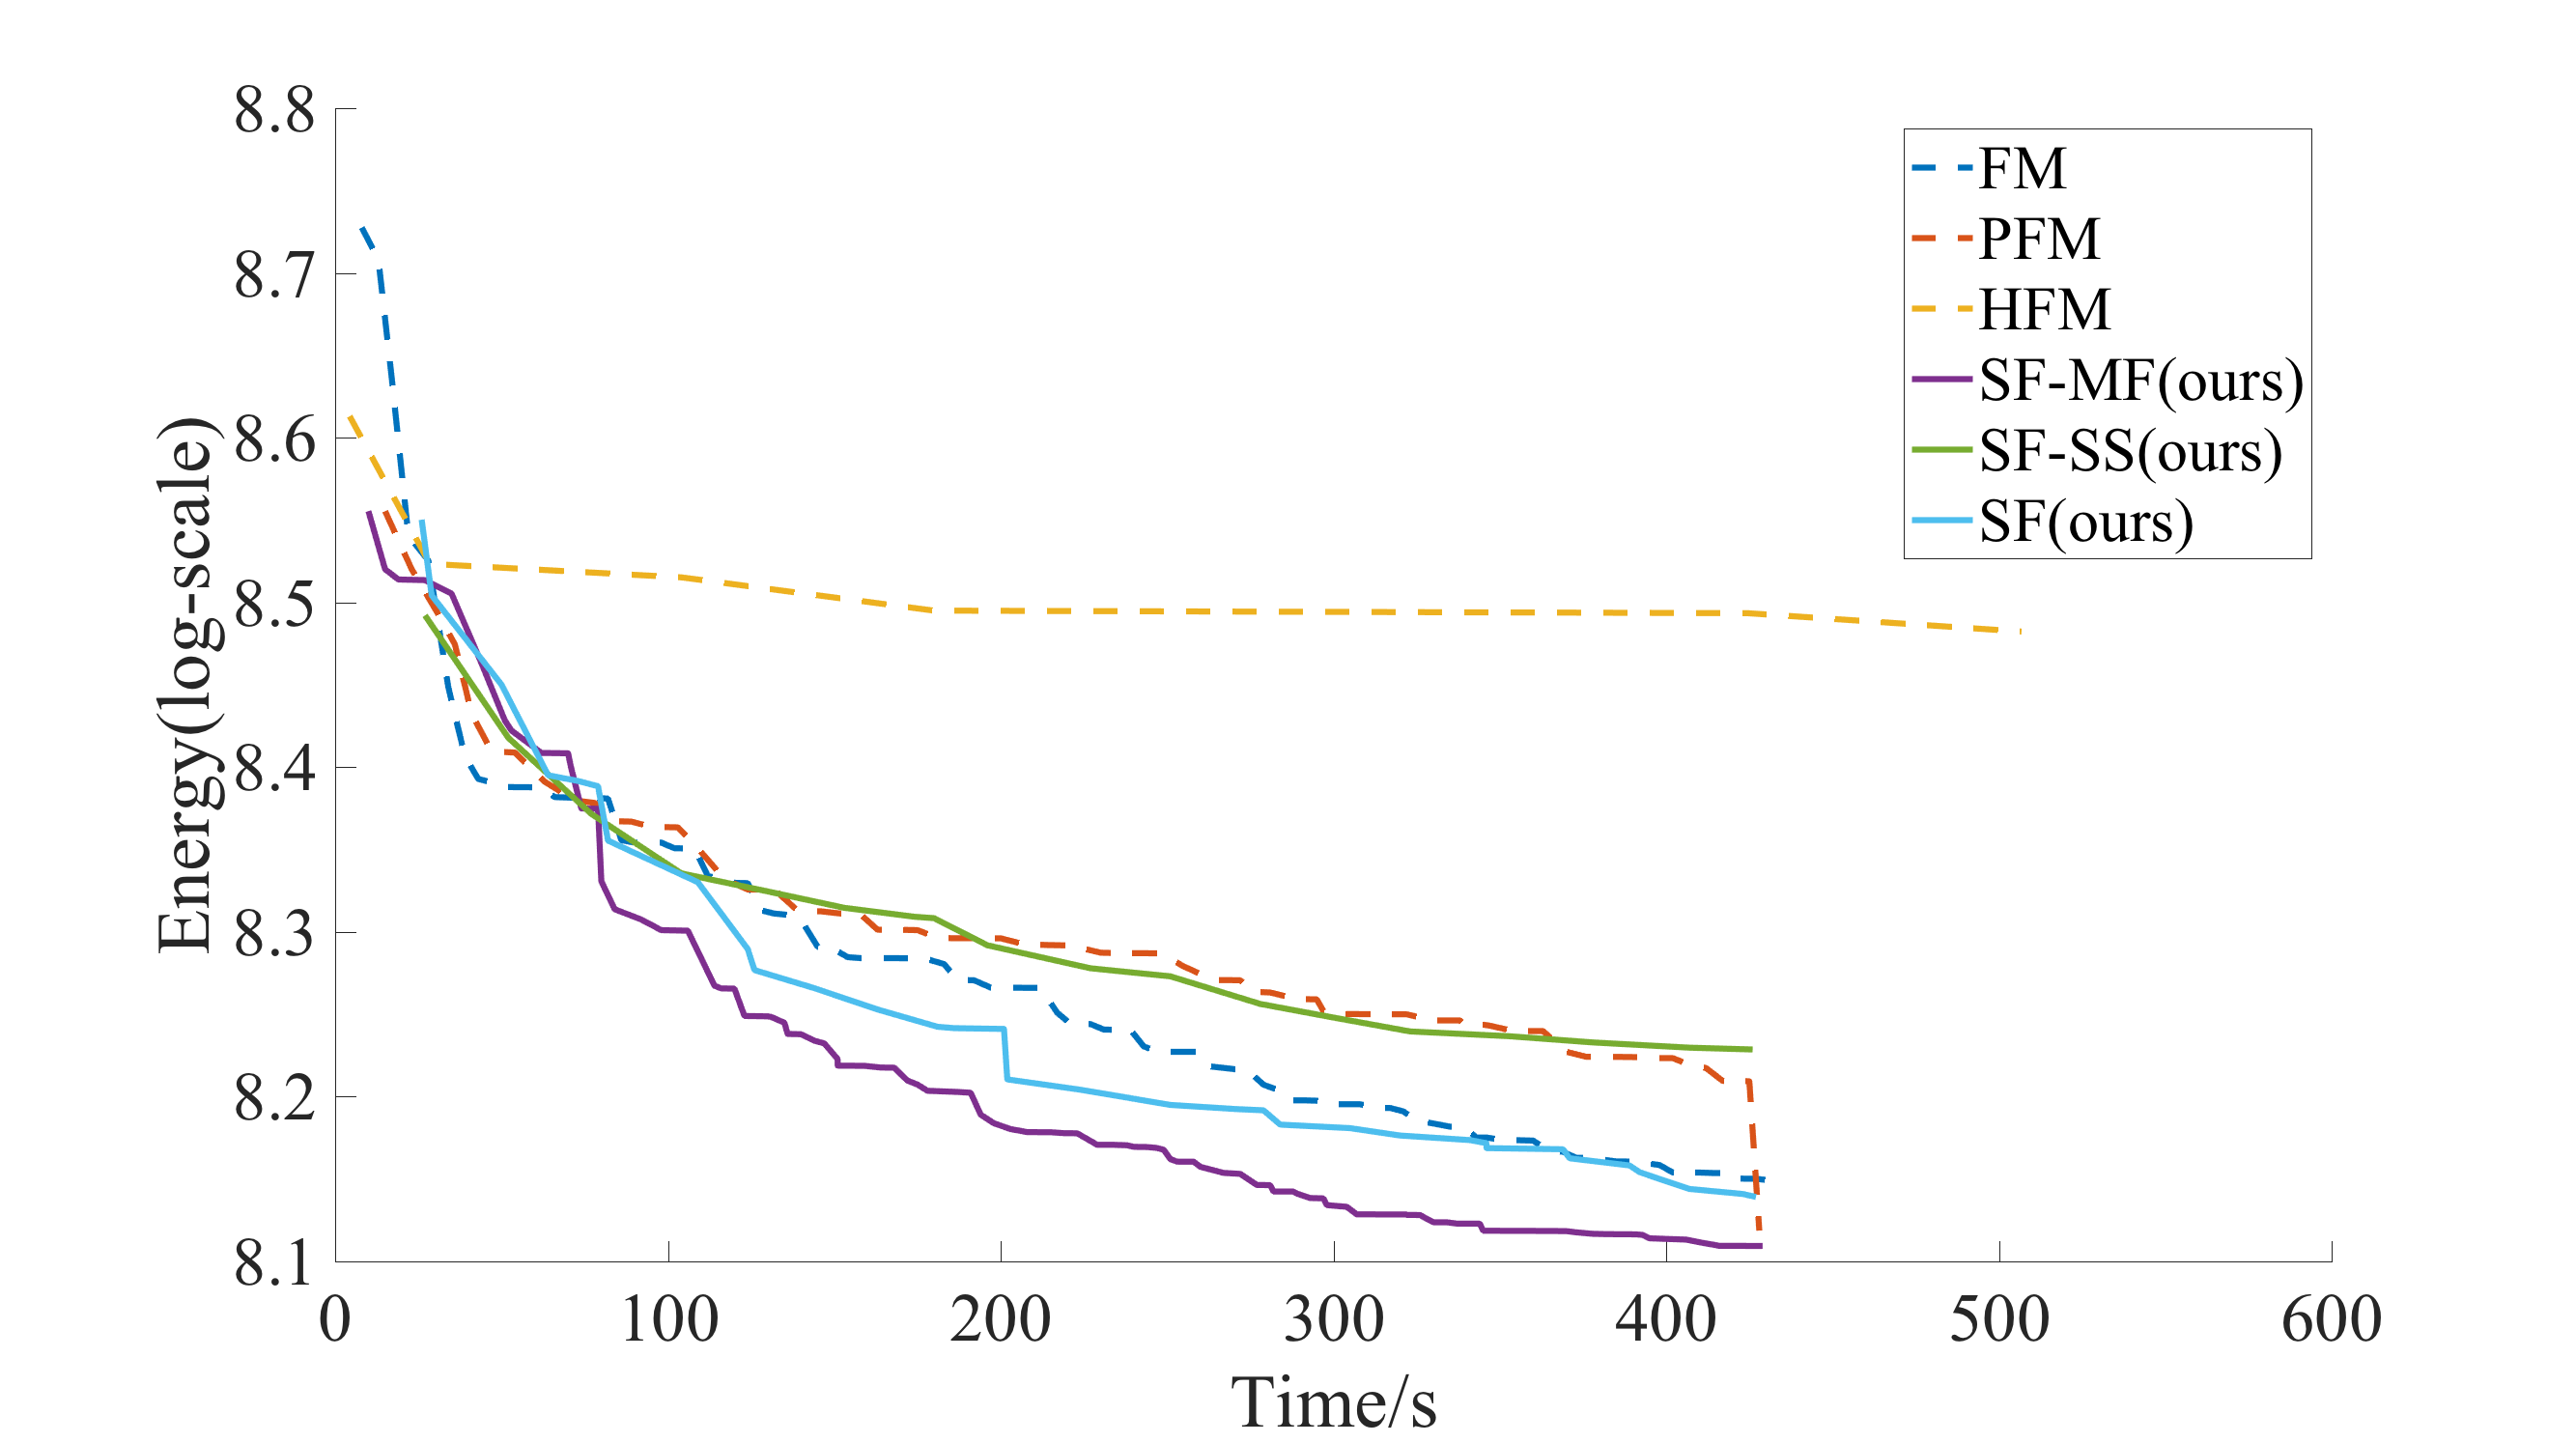
\includegraphics[width=0.8\columnwidth]{figure/optical_flow_convergence.png}
  \caption{Energy plots for optical flow estimation. SF-MF has the best
 performance due to its solution sharing strategy.}\label{fig:optical_flow_convergence}
\end{figure}

\begin{figure}[!h]
  \centering
  \begin{subfigure}[b]{0.49\columnwidth}
    \centering
    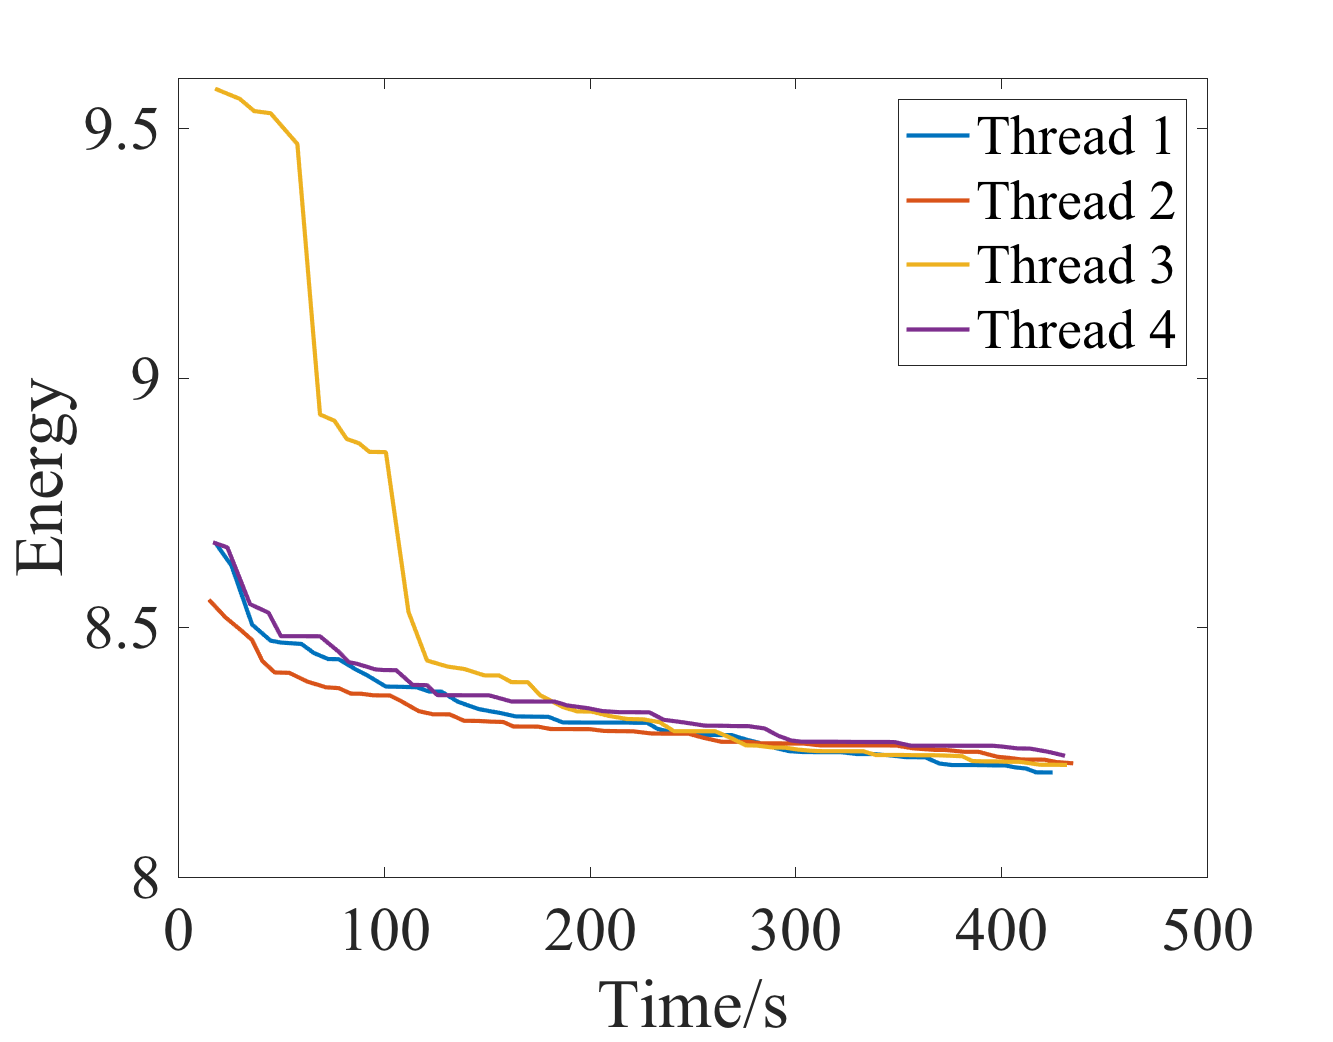
\includegraphics[width=\columnwidth]{figure/optical_flow_PFM_threads.png}
    \caption{}
    \label{fig:optical_flow_PFM_threads}
  \end{subfigure}  
  \begin{subfigure}[b]{0.49\columnwidth}
    \centering
    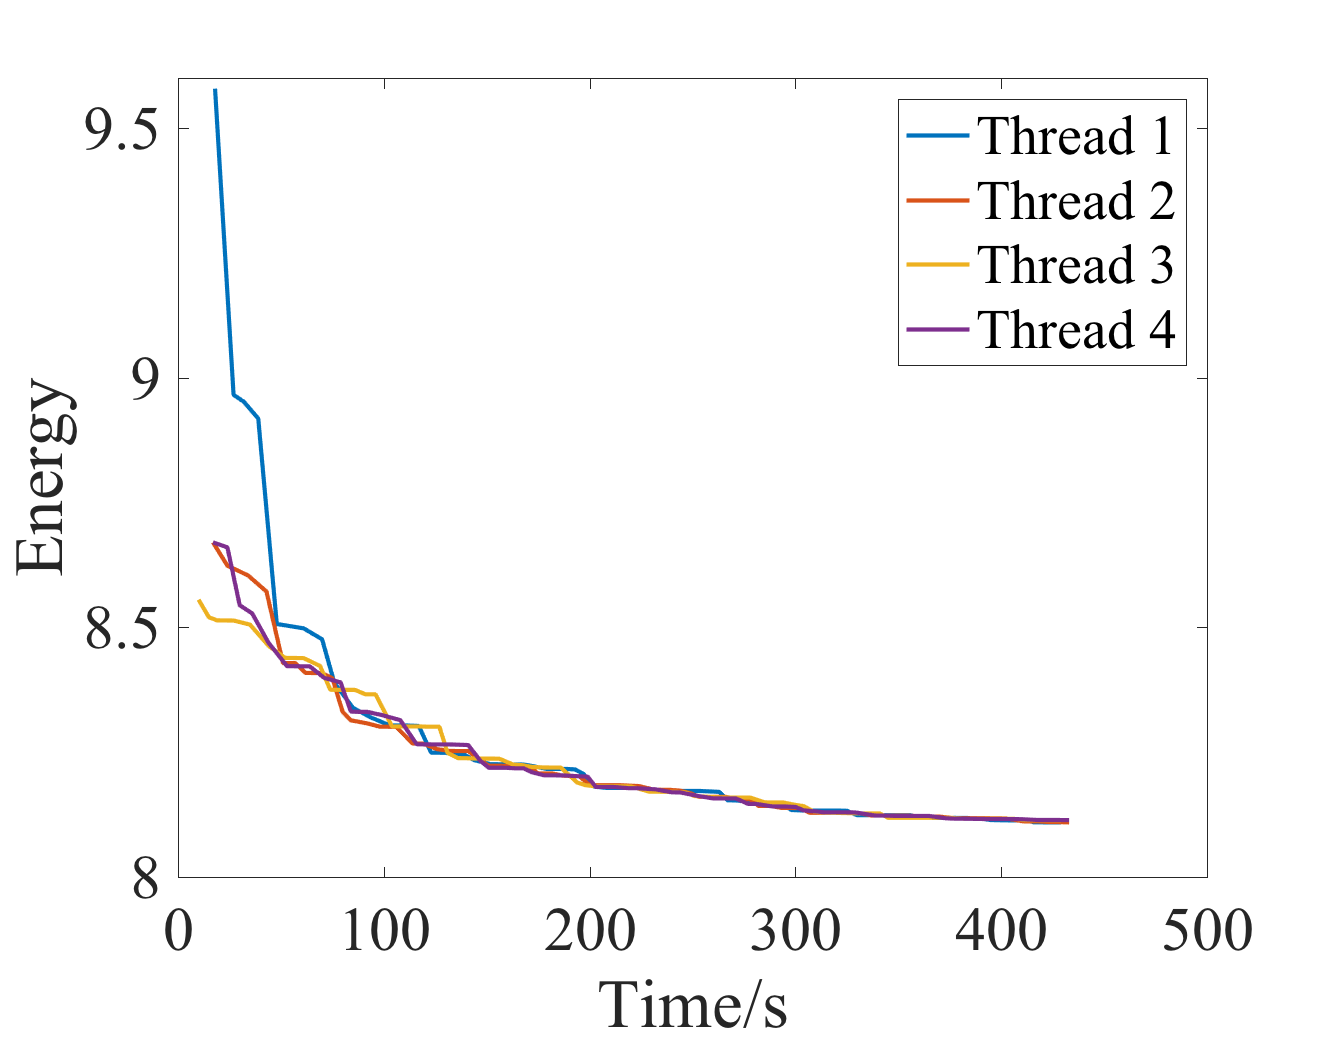
\includegraphics[width=\columnwidth]{figure/optical_flow_SF_MF_threads.png}
    \caption{}
    \label{fig:optical_flow_SF_MF_threads}
  \end{subfigure}
  \caption{Energy plots per thread for (a) Parallel Fusion  
    Move (PFM) and (b) our FS-MF.}
  \label{fig:optical_flow_by_threads}  
\end{figure}

% 
% This is because some solution proposals are more effective than others,
% so once a thread grabs an effective solution proposal, it find a lower
% energy quickly. Since there is no solution sharing in PFM model, other
% threads cannot share this lower energy state, and keeps working on its
% own state.
%
%On the other hand, SF-MF
%allows solution sharing, so once a thread grabs an effective solution
%proposal and moves to a lower energy state, other threads can share
%information about this lower energy state. In this manner, all threads
%contribute to further decrease of this low energy state. To further
%demonstrate what is happening here,
To further investigate the effectiveness of solution sharing,
Fig.~\ref{fig:optical_flow_by_threads} shows the energy plots of PFM
and SF-MF per thread. As evident from the plot, in PFM, one thread found
a better solution than others, but other threads keep working
independently at higher energy states. SF-MF, on the other hand,
exchanges solutions all the time, and every thread is making an effective
work in improving the solution.
%As we can see from the plots, in PFM model, one thread finds lower
%energy state faster than others, while other threads keep working at
%their own energy state. But in SF-MF model, all threads exchange
%information about the lowest energy state frequently and work on
%improving the lowest energy state together. Since the solution for
%optical flow can be locally improved by each thread, the final merging
%of PFM can effectively fuse good local results in different threads
%together and achieve a similar energy state with SF-MF model. But as
%SF-MF model shares information in the middle, a final merging becomes
%less necessary.
Another key finding from Fig.~\ref{fig:optical_flow_convergence} is that
SF is slower than SF-MF. Our analysis is that multi-way fusion is
inefficient in this problem setting, since solution proposals are
relatively independent and fusing the solution space would not gain much
benefit. It rather loses performance against QPBO~\cite{QPBO} due to the
overhead of TRW-S.

There are two factors influencing solution sharing: 1) \textit{the
number of solutions to share} and 2) \textit{the frequency of solution
sharing}. Both factors are controlled by $\beta$. As mentioned in
Section~\ref{section:algorithm}, we have used $\beta = 1$ (i.e., share
solutions) once in every five iterations.  To further understand the
effects of solution sharing, we did two more experiments. First, we set
$\beta$ to 0, 1, 2, or 3 in every five iterations,
% (when $\beta = 0$, it is the same with PFM without final merging).
while keeping all other parameters the same (See
Fig.~\ref{fig:optical_flow_by_beta}).  Second, we change the number of
iterations $k$ between the two consecutive solution sharing iterations
(See Fig.~\ref{fig:optical_flow_by_interval}).  The first experiment
revealed that the solution sharing makes convergence faster regardless of
$\beta$.  However, too much solution sharing slows down the convergence,
and $\beta=1$ is the sweet spot for this problem.
%
% , energy generally
% decreases faster with solution sharing. But since we need to perform one
% fusion for sharing each solution, sharing more solution decreases
% efficiency in this problem setting. While sharing multiple solutions
% might be useful in some other problem setting as it means each thread
% can get more global information early.
%
The second experiment has shown that too frequent solution sharing
harms the convergence, simply because we have less time generating more
proposals and exploring the solution space.
% From this figure, we can see that
% although solution sharing generally speeds up the optimization process,
% sharing solution too frequently is not a good practice. This is because
% when we share solution frequently, we have less time for generating and
%fusing new proposals.
Optimal parameter setting depends on each problem setting.
%A good choice of the solution sharing frequency depends on specific
%problem setting.


\begin{figure}[!h]
  \centering
  \begin{subfigure}[b]{0.49\columnwidth}
    \centering
    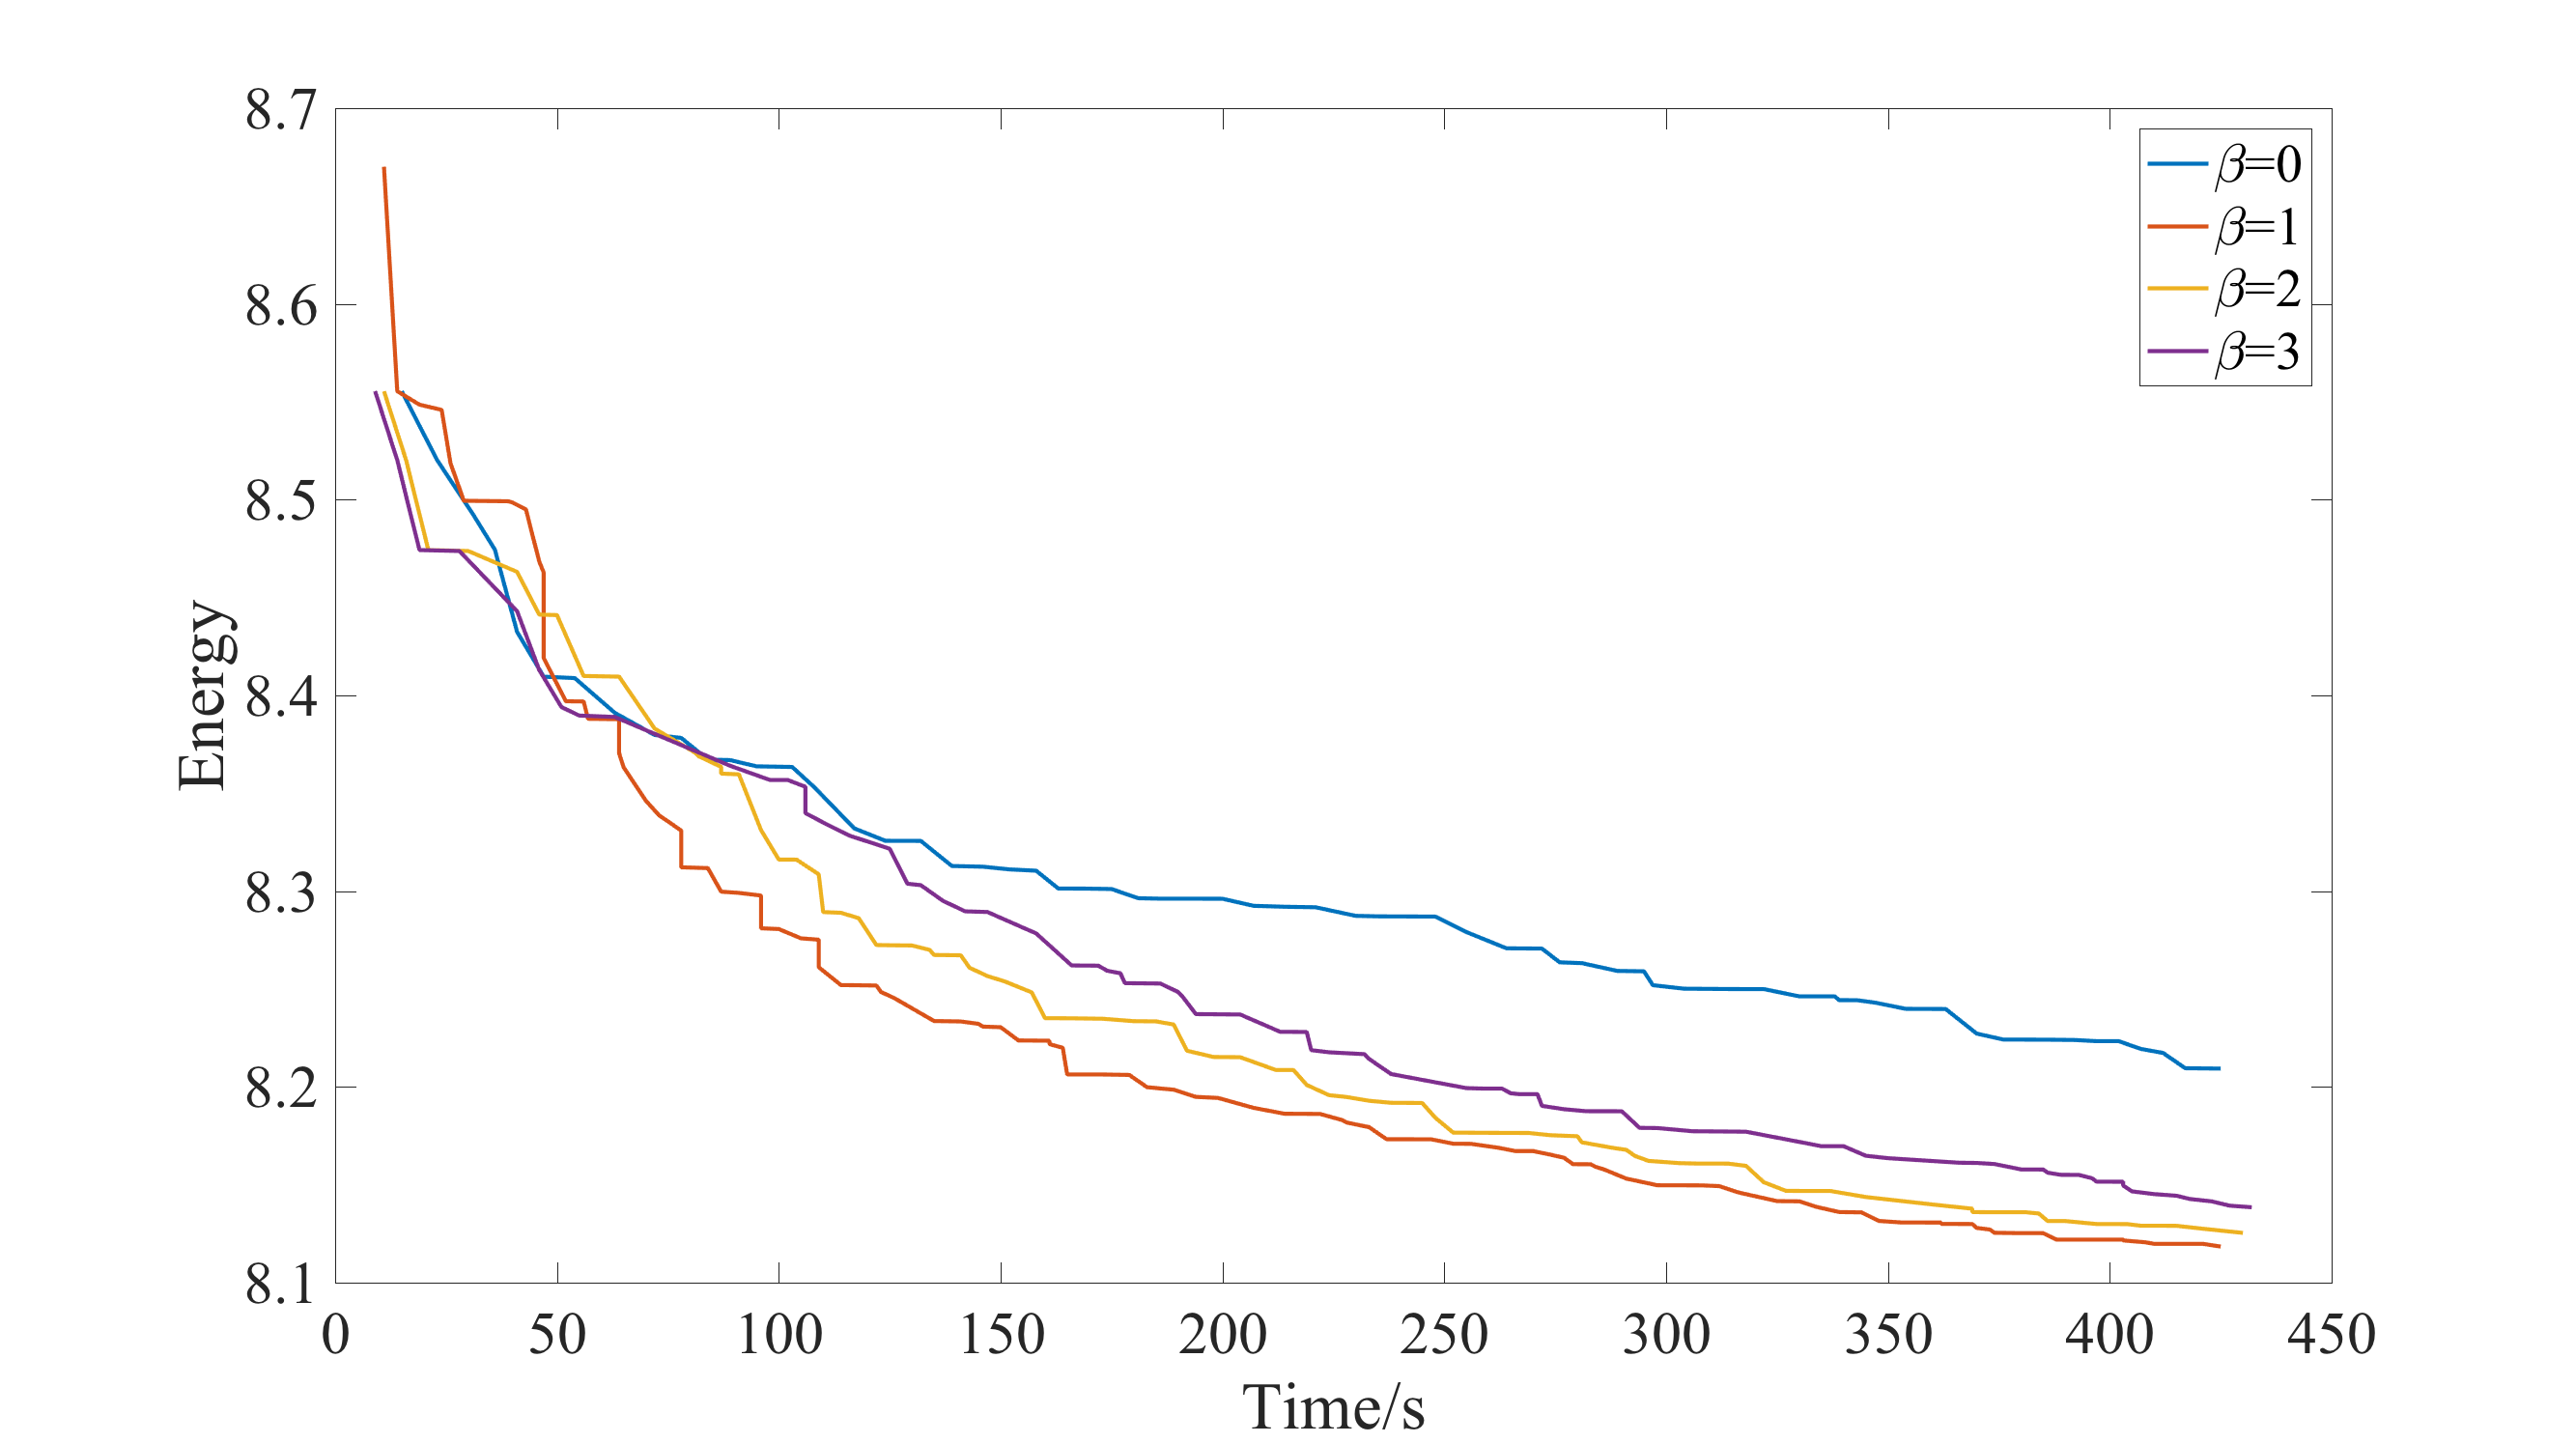
\includegraphics[width=\columnwidth]{figure/optical_flow_by_beta.png}
    \caption{}
    \label{fig:optical_flow_by_beta}
  \end{subfigure}  
  \begin{subfigure}[b]{0.49\columnwidth}
    \centering
    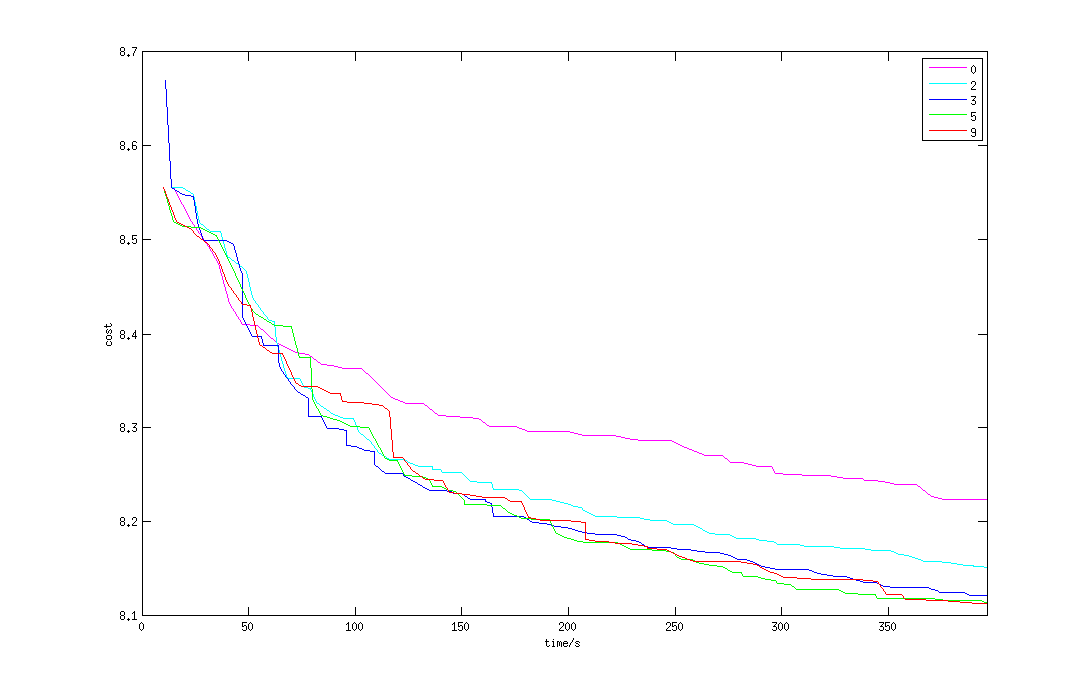
\includegraphics[width=\columnwidth]{figure/optical_flow_by_interval.png}
    \caption{}
    \label{fig:optical_flow_by_interval}
  \end{subfigure}
  \caption{Energy plots for optical flow with (a) varying
    $\beta$ and (b) varying solution sharing
    frequencies. Solution sharing achieves better convergence, but sharing too many solutions (larger $\beta$) or sharing solutions too frequently (less $k$) slows down the convergence, as it reduces the time for exploration.}
\end{figure}
